\section{Melhorias das medidas ICTs - LI, TB e TS}

% * 2024-05-13-SI_ICTs (ict-tests)


\begin{frame}{Melhorias das medidas ICTs - LI, TB e TS}

{\footnotesize
% \vspace{-0.3cm}
\begin{itemize}
    % \setlength\itemsep{1em}
    \item estudo dia 2024-05-13
    \item levantamos as curvas de carga nos ICTs do LI (osc.) x tensão de bias no EGun, antes e depois do splitting para as eletrônicas Bergoz.
    \item com o sinal das eletrônicas bergoz ativos, comparação bergoz/osciloscópio durante turno de usuário.
    \item medidas de resistência, de aterramento e ruídos (Carlos)
\end{itemize}
}
% \vspace{-0.2cm}
\begin{figure}[ht]
    \begin{minipage}[b]{0.4\linewidth}
        \centering
        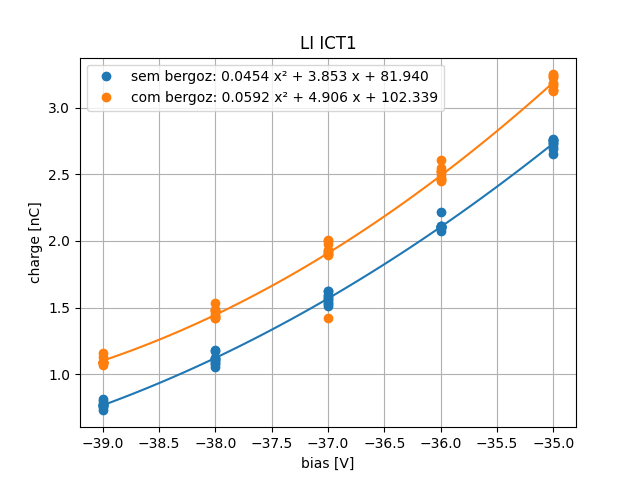
\includegraphics[width=\textwidth]{2024-07-12/figures/li-ict1.png}
        \caption{Calibration of LI ICT1.}
        \label{fig:a}
    \end{minipage}
    \hspace{0.2cm}
    \begin{minipage}[b]{0.4\linewidth}
        \centering
        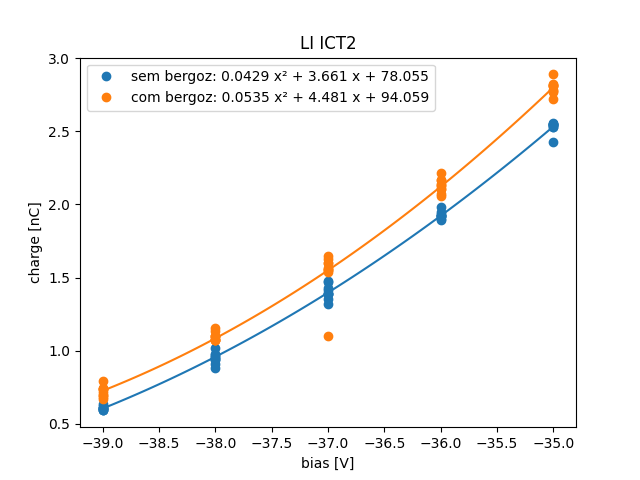
\includegraphics[width=\textwidth]{2024-07-12/figures/li-ict2.png}
        \caption{Calibration of LI ICT2.}
        \label{fig:b}
    \end{minipage}
\end{figure}
\end{frame}


% \begin{frame}{Melhorias dos ICTs do LI, TB e TS}
% \vspace{0.2cm}
% Medidas de resistência de aterramento
% \vspace{0.2cm}
% {\footnotesize
% \begin{itemize}
%     \setlength\itemsep{1em}
%     \item Entre barras de aterramento no LI, 1 Ohm,
%     \item Entre barras e estrutura aceleradora, oscilando em torno de 1.2 Ohm
%     \item A barra de aterramento próxima ao BPM 1-02 da TB não há nada conectado a ela e ela também não está aterrada.
%     \item As medidas de resistência da câmara do booster em relação ao aterramento variam em torno 1.4 Ohm em trechos distintos 
% aumentando até 6 Ohm quando se afasta do trecho de injeção, onde os magnetos pulsados estão conectados ao aterramento.
%     \item Próximo ao trecho 04 do anel, tem um cabo que vem da sala de racks e está conectado ao aterramento sem um terminal, parecendo
%     precária a conexão.
%     \item A resistência entre anel e booster, variam entre 2 e 6 Ohm, diminuindo nas proximidades onde o booster está aterrado.
% \end{itemize}
% }
% \end{frame}


% \begin{frame}{Melhorias dos ICTs do LI, TB e TS}
% \vspace{0.2cm}
% Ruídos... Fizemos diversas medidas do ruído induzido pelo septum, e os ICT's:
% \vspace{0.2cm}
% \begin{itemize}
%     \setlength\itemsep{1em}
%     \item Desconectamos o cabo de cada ICT separadamente, com o ímã pulsando e nenhum sinal do pulsador foi observado, conectando
%     ou não ma malha externa do cabo coaxial. Mostrando que não é um sinal irradiado.
%     \item Deconectamos todos os cabos inclusive os de sincronismo e conexão com a ethernet, e o sinaldo pulsador pode ainda ser observado
% \end{itemize}
% \end{frame}